% Chapter 3 - Methodology
% With Sample Figures From Kevin Hughes

\glsresetall % reset the glossary to expand acronyms again
\chapter[Methodology]{Methodology and Design}\label{ch:Methodology}
\index{Methodology}

This chapter details the design and engineering decisions taken to develop and evantually implement digitising ECG signals through mobile applications. These decisions are guided by the observations highlighted in the \href{ch:LitReview}.

It will begin with a highlevel overview of the proposed approach for tackling the problem. It will then provide specific details on the methods and techniques used in the research, including any algorithms, tools, and technologies employed. The chapter will also discuss the rationale behind these choices, highlighting how they align with the research objectives and address the identified challenges.

%-------------------------------------------------------

\section{Overview of Approach}

The core principle of the proposed approach is iteration. With each new stage of development, earlier steps are revisited to ensure ongoing risk management and continuous improvement. This cyclical process mirrors the spiral model commonly applied in system and software design.

\begin{figure}[H]
    \centering
    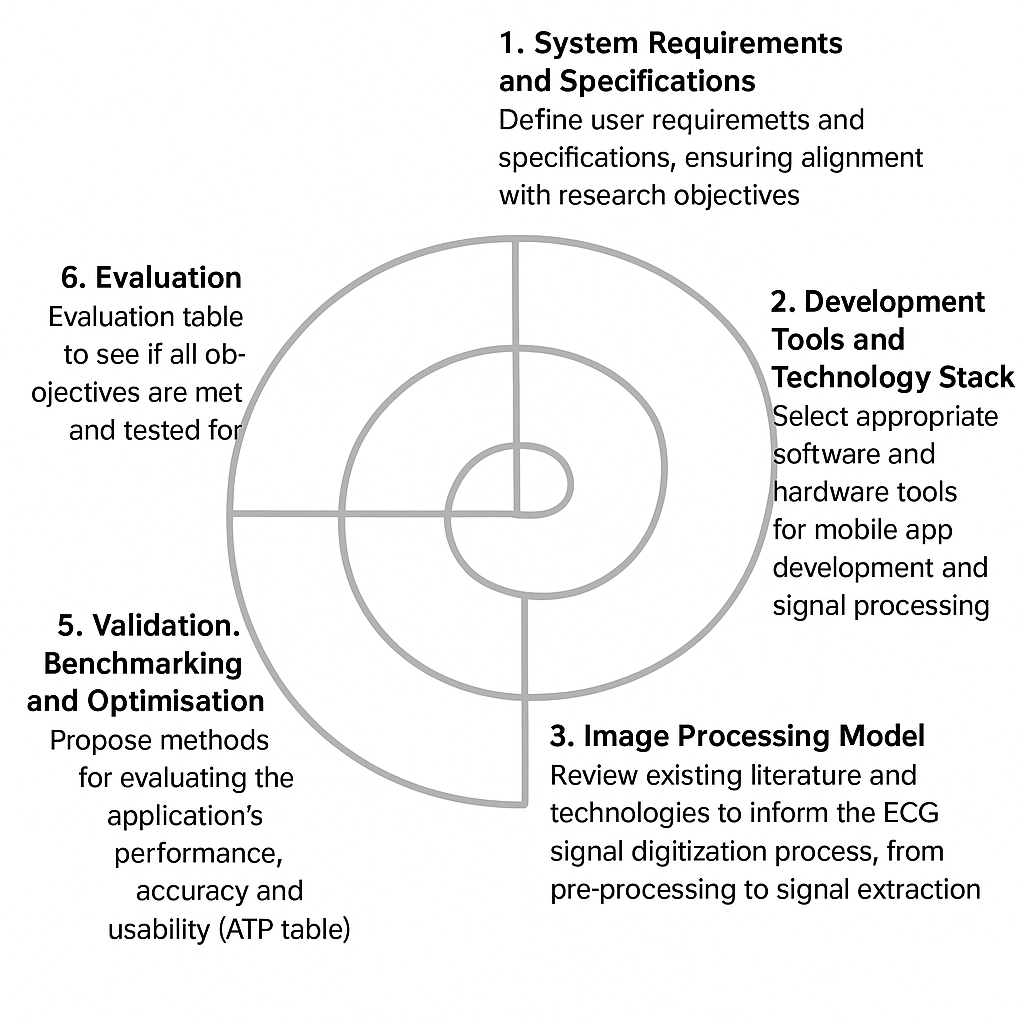
\includegraphics[width=0.7\textwidth]{3_Chapters/3_Chapter_Methodology/Figures/Spiral Model.png}
    \caption{Spiral Model of Development}
    \label{fig:SpiralModel}
\end{figure}

\begin{enumerate}
	\item \textbf{System Requirements and Specifications:} Define user requirements and specifications, ensuring aignment with research objectives
	\item \textbf{Development Tools and Technology Stack:} Select appropriate software and hardware tools for mobile app development and signal processing
	\item \textbf{Image Processing Model:} Review existing literature and technologies to inform the ECG signal digitisation process, from pre-processing to signal extraction
	\item \textbf{Design and Prototyping:} Create iterative versions of the mobile application to test core functionalities, using wireframes for illustration
	\item \textbf{Validation, Benchmarking, and Optimisation:} Propose methods for evaluating the application's performance, accuracy, and usability (ATP table)
	\item \textbf{Evaluation:} Evaluation table to see if all objectives are met and tested for
\end{enumerate}

%---------------------------------------------------------

\section{System Requirements and Specifications}

The objectives of the research are clear: design a mobile application (Android or iOS) that can (1) facilitate the capturing of ECG paper records, (2) process the captured images to extract the ECG waveform, and (3) store the digitised ECG signals in a standardised digital format. The following user and functional requirements and specifications are derived from these objectives. 

\subsection{Functional User Requirements}

\begin{table}[H]
	\centering
	\caption{Functional User Requirements}\label{tab:UserReq}
    \begin{tabular}{l|l|p{9.5cm}}
    \hline
    \textbf{\#no.} & \textbf{Requirement}       & \textbf{Description}                                                                    \\
	\hline
    FR01  & Camera Access     & Application must be able to access the mobile's camera                         \\
    FR02  & Image Import      & Access photo library for image upload                                          \\
    FR03  & Pre-processing    & Must facilitate cleaning and aligning of image for signal extraction           \\
    FR04  & Signal extraction & Detect signal and extract it in pixel coordinates                              \\
    FR05  & Reconstruction    & Convert pixel coordinates to amplitude-time series                             \\
    FR06  & Data storage      & Facilitate storing of digitised data in external device or cloud in CSV format \\
    FR07  & Visualisation     & Display interactive ECG waveform                                               \\
	\hline
    \end{tabular}
\end{table}

\subsection{Non-Functional User Requirements}

\begin{table}[H]
	\centering
	\caption{Non-Functional User Requirements}\label{tab:NonFuncReq}
    \begin{tabular}{l|l|p{9.5cm}}
    \hline
    \textbf{\#no.} & \textbf{Requirement}       & \textbf{Description}                                                   \\
	\hline
    NFR01 & Performance         & Image capture and signal extraction should complete within acceptable time ($<$ 5 sec) \\
    NFR02 & Accuracy            & Maintain reliable signal extraction across various ECG paper qualities              \\
    NFR03 & Usability           & Interface must be simple, clear, and intuitive for users with minimal training      \\
    \hline
    \end{tabular}
\end{table}

\begin{table}[H]
	\centering
    \begin{tabular}{l|l|p{9.5cm}}
    \hline
    NFR04 & Reliability         & Handle errors gracefully and allow retry; ensure data persists between sessions     \\
    NFR05 & Compatibility       & Support Android or iOS devices with standard camera specifications                 \\
    NFR06 & Security 			& Store data securely on device; optionally encrypt sensitive information             \\
	\hline
    \end{tabular}
\end{table}

%---------------------------------------------------------

\section{Tools and Technology Stack}

Defining the development environment for any software project is crucial, as it influences the efficiency of the development process, the quality of the final product, and the ease of maintenance. This section outlines the chosen tools and technologies for developing the mobile application for digitising ECG signals. Notice that the chosen operating system is iOS because of its comprehensive set of libraries and frameworks for image processing through Xcode.

\subsection{Development Tools and Specifications}

\begin{itemize}
    \item \textbf{Xcode:} The integrated development environment (IDE) for macOS, used for developing software for iOS. It provides a suite of tools for designing user interfaces, writing code, and debugging applications.
    \item \textbf{Apple Developer:} A platform that provides resources and tools for iOS app development, including access to beta software, advanced app capabilities, and app analytics. This is essential for deploying to a physical iOS device for testing through Testflight.
    \item \textbf{Simulator:} A tool within Xcode that allows developers to test and debug iOS applications on a Mac without needing a physical device. It simulates various iPhone and iPad models and iOS versions.
    \item \textbf{iPhone 13:} A physical device used for testing the application in real-world conditions, ensuring that it performs as expected on actual hardware and observing real user interactions.
    \item \textbf{VMware Workstation Pro:} A virtualisation software used to run macOS on a Windows machine, enabling the use of Xcode and other macOS-specific tools without needing a dedicated Mac. It provides a controlled environment for iOS development and testing. The specfic macOS installed is Sequioa, running on a Mac Mini 4. For compatibility with the Windows PC, the virtual machine is allocated 4GB RAM, 4 CPU cores and 128GB of disk space.
\end{itemize}

\subsection{Technology Stack}

\textbf{iOS SDK}   
The iOS SDK is Apple’s official development toolkit for building applications on iPhones and iPads. It provides access to the operating system’s APIs, device hardware (camera, sensors, storage), and system-level services. This research project requires close integration with the iPhone camera for ECG capture, efficient on-device signal processing, and secure file handling. The iOS SDK ensures native access to all necessary features while maintaining compliance with Apple’s ecosystem.  

It provides a complete and unified set of frameworks for image processing, file management, and graphics rendering, while being ptimized for Apple hardware, ensuring smooth performance and efficient energy usage. It offers long-term reliability and stability since it is fully supported by Apple.  

\begin{itemize}
    \item \textbf{Security:}  Applications built with the iOS SDK run in a sandboxed environment, preventing unauthorized access to other apps or system files. It supports data encryption at rest and in transit, aligning with healthcare data protection needs (e.g., HIPAA compliance). It requires that all apps be \textbf{digitally signed}, which ensures authenticity and protects users from tampered or malicious code.  
    \item \textbf{Performance:} The SDK provides frameworks (e.g., Core Image, Accelerate) that are hardware-accelerated using the CPU, GPU, and Neural Engine. It ensures real-time responsiveness, critical for ECG pre-processing and visualization tasks. The native compilation reduces overhead compared to cross-platform solutions, leading to faster execution and lower battery drain.  
    \item \textbf{Integration:} The SDK seamlessly integrates with device features such as the camera, storage, sensors, and security mechanisms. Furthermore, it provides compatibility with higher-level frameworks such as Core Image (image processing), Vision (computer vision), and CloudKit (cloud storage). It as well ensures consistent user experience by adhering to iOS UI/UX design standards.
\end{itemize}

\textbf{Core iOS Frameworks and Libraries}

\begin{itemize}
    \item \textbf{Core Image:} Apple’s image processing framework designed for filtering, noise reduction, normalization, and geometric corrections such as dewarping ECG scans. It uses GPU acceleration, allowing fast and energy-efficient processing on mobile hardware. Core Image can work in parallel with Vision to prepare images for further feature extraction.  
    \item \textbf{Vision Framework:} A high-level computer vision framework for feature detection, object recognition, and image alignment. Vision is useful for detecting ECG grid lines and aligning the paper image before signal extraction. It complements Core Image by handling structural analysis while Core Image focuses on pixel-level filtering.  
    \item \textbf{Accelerate Framework:} A low-level framework that provides optimized mathematical, signal processing, and digital signal processing (DSP) functions. It uses vectorization and hardware acceleration (CPU and GPU) to speed up operations. This is crucial for transforming images into ECG signals, and it often works in sequence after preprocessing by Core Image and Vision.  
    \item \textbf{Foundation Framework:} A system-level framework that provides essential services such as data structures, file management, and I/O operations. It is used for generating and managing CSV files that store the extracted ECG time-series data. Its advantage lies in efficiency and reliability when handling structured data within the iOS environment.  
    \item \textbf{Core Graphics / Quartz 2D:} A two-dimensional rendering engine that allows vector-based and pixel-accurate drawing. It is used in DigECG to visualize ECG waveforms on the app’s interface. This framework complements Accelerate, where Accelerate computes the signal data and Core Graphics ensures precise visual representation.  
\end{itemize}

\textbf{External Tools for Benchmarking and Evaluation}

\begin{itemize}
    \item \textbf{OpenCV:} An open-source computer vision library that provides a wide range of algorithms for image segmentation, edge detection, and noise removal. OpenCV is advantageous for prototyping and experimentation, as it offers robust tools not natively available in iOS. In DigECG, it was used in parallel with Core Image and Vision during development to validate preprocessing accuracy and ensure robustness under varied conditions.
    \item \textbf{MATLAB:} A high-level scientific computing environment with specialized toolboxes for biomedical signal processing and analysis. MATLAB was used to benchmark ECG extraction accuracy against ground truth datasets, and to apply advanced filtering and spectral analysis. It complements OpenCV by focusing on quantitative evaluation of the extracted signals, ensuring that image-to-signal conversion methods in the app are scientifically validated.  
\end{itemize}

\textbf{Cloud Integration}

\begin{itemize}
    \item \textbf{CloudKit:} Apple’s cloud service framework for storage and synchronization across devices. CloudKit provides end-to-end encryption and secure authentication, making it suitable for sensitive healthcare data. For DigECG, it is planned as an extension to store digitized ECG files securely, ensuring data is not only stored locally but also accessible across devices for patient monitoring and medical record keeping. This complements local CSV file storage by adding reliability and redundancy through cloud backup.  
\end{itemize}
%---------------------------------------------------------

\section{Image Processing Model}

In this section, the observations from the liteature will be used to draw up and choose a model for the image processing required for digitising the ECG signal.

%---------------------------------------------------------

\section{Design and Prototyping}

Prototyping bridges the conceptualisation of the app and its realisation. Low-fidelity wireframes are used to outline structure, navigation, and features. Iterative refinements ensure usability and alignment with requirements.

\subsection{Wireframes}

\subsubsection{Home / Dashboard Wireframe}
\textbf{Purpose:} Navigation hub.

\textbf{Features:}
\begin{itemize}
    \item Upload/scan ECG image.
    \item Access recent digitised signals.
    \item Settings (signal scaling, export formats).
\end{itemize}

\subsubsection{Image Pre-processing Screen Wireframe}
\textbf{Purpose:} Present uploaded ECG scan and allow preprocessing. 

%I would like to automate this BUT keeping this here for incase
\textbf{Features:}
\begin{itemize}
    \item Toggle grid removal.
    \item Noise reduction preview.
    \item Region-of-interest selection.
    \item Undo/redo controls.
\end{itemize}

\subsubsection{Signal Extraction Screen Wireframe}
\textbf{Purpose:} Display detected ECG trace.  

\textbf{Features:}
\begin{itemize}
    \item Overlay of raw scan and extracted waveform.
    \item Baseline correction adjustments.
    \item Manual correction tools (erase/add points).
\end{itemize}

\subsubsection{Signal Reconstruction \& Visualisation Wireframe}
\textbf{Purpose:} Display reconstructed digital ECG waveform

\textbf{Features:}
\begin{itemize}
    \item Interactive graph (zoom, pan, scale).
    \item Lead/time scaling indicators (mm/s, mV).
    \item Resampling and export options.
\end{itemize}

\subsubsection{Export / Results Screen Wireframe}
\textbf{Purpose:} Final storage and sharing stage

\textbf{Features:}
\begin{itemize}
    \item Export options (CSV, JSON, MATLAB, PDF).
    \item Share via email/cloud.
    \item Comparison view (digitised vs raw scan).
\end{itemize}

\subsection{Iterations}
The initial prototype offered only ... 

Iterations added:
\begin{itemize}
    \item Preprocessing toggles (grid/noise removal).
    \item Manual correction tools for overlapping artifacts.
    \item Interactive waveform viewer (zoom, pan, scaling).
    \item Multiple export formats.
\end{itemize}

\subsection{User Flow}

\subsubsection{Home Screen}
\begin{itemize}
    \item Case 1: Upload or capture ECG.
    \item Case 2: Access recent digitised signals.
    \item Case 3: Open settings for scale and export configuration.
\end{itemize}

\subsubsection{Pre-processing Screen}
\begin{itemize}
    \item Case 1: Apply automatic grid removal. (maybe remove in other iterations - can be a base)
    \item Case 2: Apply artifact filtering.
    \item Case 3: Select ECG region of interest or entire ECG. 
\end{itemize}

\subsubsection{Signal Extraction Screen}
\begin{itemize}
    \item Case 1: View automatically extracted waveform.
    \item Case 2: Manually adjust trace (add/remove points).
    \item Case 3: Re-run extraction with different thresholds.
\end{itemize}

\subsubsection{Signal Reconstruction \& Visualisation}
\begin{itemize}
    \item Case 1: View digitised ECG in interactive graph.
    \item Case 2: Compare digitised vs raw waveform overlay.
    \item Case 3: Adjust scaling (25 mm/s, 10 mm/mV).
\end{itemize}

\subsubsection{Export Screen}
\begin{itemize}
    \item Case 1: Save waveform as CSV.
    \item Case 2: Export as PDF overlay.
    \item Case 3: Share via cloud/EHR system.
\end{itemize}


\section{Validation, Benchmarking, and Optimisation}

\section{Evaluation}
